\chapter{Elliptic curves}
\label{cha:EC}
In this chapter we define elliptic curves and present results which will be useful. One can consider this chapter as a toolbox for later. 
\section{Definition of an elliptic curve}
\label{sec:defEC}
%\section{Projective space}
%\label{sec:projectiveSpace}
Let $\F$ be an arbitrary field and put $f(x,y)=ax^3+bx^2y+cxy^2+dy^3+ex^2+fxy+gy^2+hx+iy+j$. If at least one of $a,b,c,d$ is non-zero then
\begin{align}\label{affineEC}
	f(x,y)=0
\end{align}
is a degree 3 curve in $\F^2$ with affine solutions $(x,y)\in \F^2$. If we homogenize $f$ we have $F(x,y,z)=ax^3+bx^2y+cxy^2+dy^3+ex^2z+fxyz+gy^2z+hxz^2+iyz^2+jz^3$ and the projective form of (\ref{affineEC}) is then
\begin{align}\label{projectiveEC}
	F(x,y,z)=0.
\end{align}
This curve has the solutions $(x,y,z)\in \F^3$. Notice that if $(x,y,z)$ is an solution with $(x,y,z)\neq(0,0,0)$ then so is $(\alpha x, \alpha y, \alpha z)$ for any $\alpha\in\F^*$. Hence it makes more sense to talk about solutions to (\ref{projectiveEC}) as being in the projective space $\P^2(\F)$. Recall that the projective space $\P^2(\F)$ consists of equivalence classes $[x,y,z]$ with respect to the equivalence relation:
\begin{align*}
	(x,y,z)\sim (x',y',z') \Leftrightarrow \exists \alpha\in \F^*:\, \alpha x=x',\, \alpha y=y',\, \alpha z=z'.
\end{align*}

The curve (\ref{projectiveEC}) is called non-singular if over $\overline{\F}$ there is no point $[x,y,z]$ on the curve (\ref{projectiveEC}) where all three partial derivatives of $F$ vanish. We are now ready to state the definition of an elliptic curve. 
\begin{defn}\label{def:ellipticCurve}
	A non-singular cubic curve of the form (\ref{projectiveEC}) with at least one rational point $(x,y,z)\in \F^3\backslash{(0,0,0)}$ is said to be an elliptic curve over $\F$.  
\end{defn}
Consider now the homogeneous equation 
\begin{align}\label{projLongW}
	y^2z+a_1xyz+a_3yz^2=x^3+a_2x^2z+a_4xz^2+a_6z^3
\end{align}
with $a_i\in\F$ for some arbitrary field $\F$. It turns out that if the defining equation (\ref{projectiveEC}) is an elliptic curve then it is birationally equivalent to (\ref{projLongW}), see \cite{milne2006}. That is, we may express all elliptic curves on the form (\ref{projLongW}). 


\section{Weierstrass model}
\label{sec:WeierstrassForm}
Assume we are given an elliptic curve of the form (\ref{projLongW}) over the field $\F$ and let $[x,y,z]$ be a point on it. Then $(x,y,z)\neq (0,0,0)$ by assumption. The points with $z=0$ are called the points at infinity. Actually we should rather say \textit{the} point at infinity; putting the point $[x,y,0]$ into (\ref{projLongW}) yield $0=x^3$ hence $x=0$. Since points are only determined up to multiplication by a unit($y\neq 0$ since $x=0=z$ and $(0,0,0)$ is excluded), $[0,1,0]$ must be the only point at infinity.

Next consider the curve 
\begin{align}\label{longW}
	y^2+a_1xy+a_3y = x^3+a_2x^2+a_4x+a_6.
\end{align}
This is called the affine part of an elliptic curve. Solutions to the above curve are embedded in the solutions for (\ref{projLongW}) by $(x,y)\mapsto [x,y,1]$. Likewise if $z\neq 0$ , a solution $[x,y,z]$ for the projective curve corresponds to the solution $(x/z,y/z)$ for the affine curve. When $z=0$, $[x,y,z]$ do not correspond to a solution on the affine curve - but there are only one of these. All points on the projective curve has the form $[x,y,1]$, except the point at infinity, so we may interpret the points on the projective curves as points $(x,y)$ satisfying (\ref{longW}) plus the point at infinity. When working with the affine part of an elliptic curve, the one point at infinity will be denoted by $\infi$.

If the curve (\ref{longW}) defines an elliptic curve it is said to be in long Weierstrass form. If $\Char(\F)\neq 2$ we may use the transformation $(x,y)\mapsto \left( x,y-\frac{a_1x+a_3}{2}\right)$ to transform the long Weierstrass form into Weierstrass form: 
\begin{align}\label{W}
	y^2=x^3+Cx^2+Ax+B,\quad A,B,C\in\F.
\end{align}
Further if $\Char(\F)\neq 2,3$ then we can transform the above curve into short Weierstrass form
\begin{align}\label{shortW}
	y^2=x^3+ax+b
\end{align}
using the transformation $(x,y)\mapsto \left(x-\frac{C}{3},y\right)$.

When we are faced with curves on the form (\ref{W}) and (\ref{shortW}) it is easy to see whether they define an elliptic curve or not; in the case of (\ref{shortW}) it defines an elliptic curve if $4a^3+27b^2\neq 0$ and (\ref{W}) defines an elliptic curve if $4A^3+27B^2-19ABC-A^2C^2+4BC^3\neq 0$.

From now on when we write elliptic curve one should think of the points on the curve (\ref{longW}) plus the point at infinity $\infi$ which is the projective point $[0,1,0]$ on the projective form of the affine curve although we will be using the projective coordinates when in practice because they induce faster addition and doubling. The special case curves (\ref{W}) and (\ref{shortW}) will be denoted $E_{W,a,b,c}$ and $E_{W,a,b}$ respectively.

\section{Group structure on elliptic curves}\label{sec:ECGroup}
\begin{defn}\label{def:setPoints}
Let $E$ be an elliptic curve curve over the field $\F$. Then $E(\F)$ denotes the set of points on $E$ plus the point at infinity. In the special cases (\ref{W}) and (\ref{shortW}) we have
\begin{align*}
E_{W,a,b,c}(\F)& =\left\{ (x,y)\in\F^2\,\vert\, y^2=x^3+cx^2+ax+b\right\}\cup\{\infi\} \\
E_{W,a,b}(\F)& =\left\{ (x,y)\in\F^2\,\vert\, y^2=x^3+ax+b\right\} \cup\{\infi\}
\end{align*} 
\end{defn}
By magic it is possible to define a composition on the set $E(\F)$ making it into a group! We restrict ourself to the case $\Char(\F)\neq 2$. It is possible to define a composition in general but it is more complicated and we do not need it. 

Let $P_1,P_2\in E_{W,a,b,c}(\F)$ (not  necessarily distinct) and write $P_1=(x_1,y_1)$ and $P_2=(x_2,y_2)$. Define the operator $\oplus$ by:
\begin{enumerate}[(1)]
\item $-\infi= \infi$
\item $-P_1=(x_1,-y_1)$
\item $\infi \oplus P_1 = P_1$
\item If $P_1 = -P_2$ then $P_1\oplus P_2=\infi$
\item If $P_1 \neq -P_2$ define
\begin{align*}
	m = \begin{cases} 
		\frac{y_2-y_1}{x_2-y_2} & x_2\neq x_1 \\
		\frac{3x_1^2+2cx_1+a}{2y_1} & x_2= x_1
		\end{cases}				
\end{align*}
then $P_1\oplus P_2=(x_3,y_3)$ with
\begin{align}
	x_3 &= m^2-c-x_1-x_2\label{add1}\\
	y_3 &= m(x_1-x_3)-y_1\label{add2}
\end{align}
\end{enumerate}
Popular $\oplus$ is also referred to as the \textit{chord-tangent construction} because of the following geometrical view: If $P_1$ and $P_2$ are distinct and not equal to $\infi$, then take the straight line trough both points and mark the third point of intersection with the curve (this point always exists unless the line is vertical in which case the sum would be the point at infinity see case 4). Take the marked point and reflect it in the $x$-axis (exists since $(x,y)\in E_{W,a,b,c}(\F)$ if and only if $(x,-y)\in E_{W,a,b,c}(\F)$) and let this be the sum of $P_1 \oplus P_2$. If the two points are equal, take the tangent to that point (this is well defined because of the non-singular condition we put on elliptic curves) and mark the third point of intersection, reflect this point in the $x$-axis and let that point be the sum $P_1\oplus P_2$. This geometrical description is a good way to visualize the composition in the case $\F=\R$ where one may draw the addition, see figure \ref{fig:dedicatedAddition} and \ref{fig:doubling}. When e.g. $\F=\Z/p\Z$ for some prime $p$ it may be confusing to try to draw the addition. In any case the composition defines a group on the set $E_{W,a,b,c}(\F)$.
\begin{figure}[htp]
\begin{minipage}[b]{0.5\linewidth}
\centering
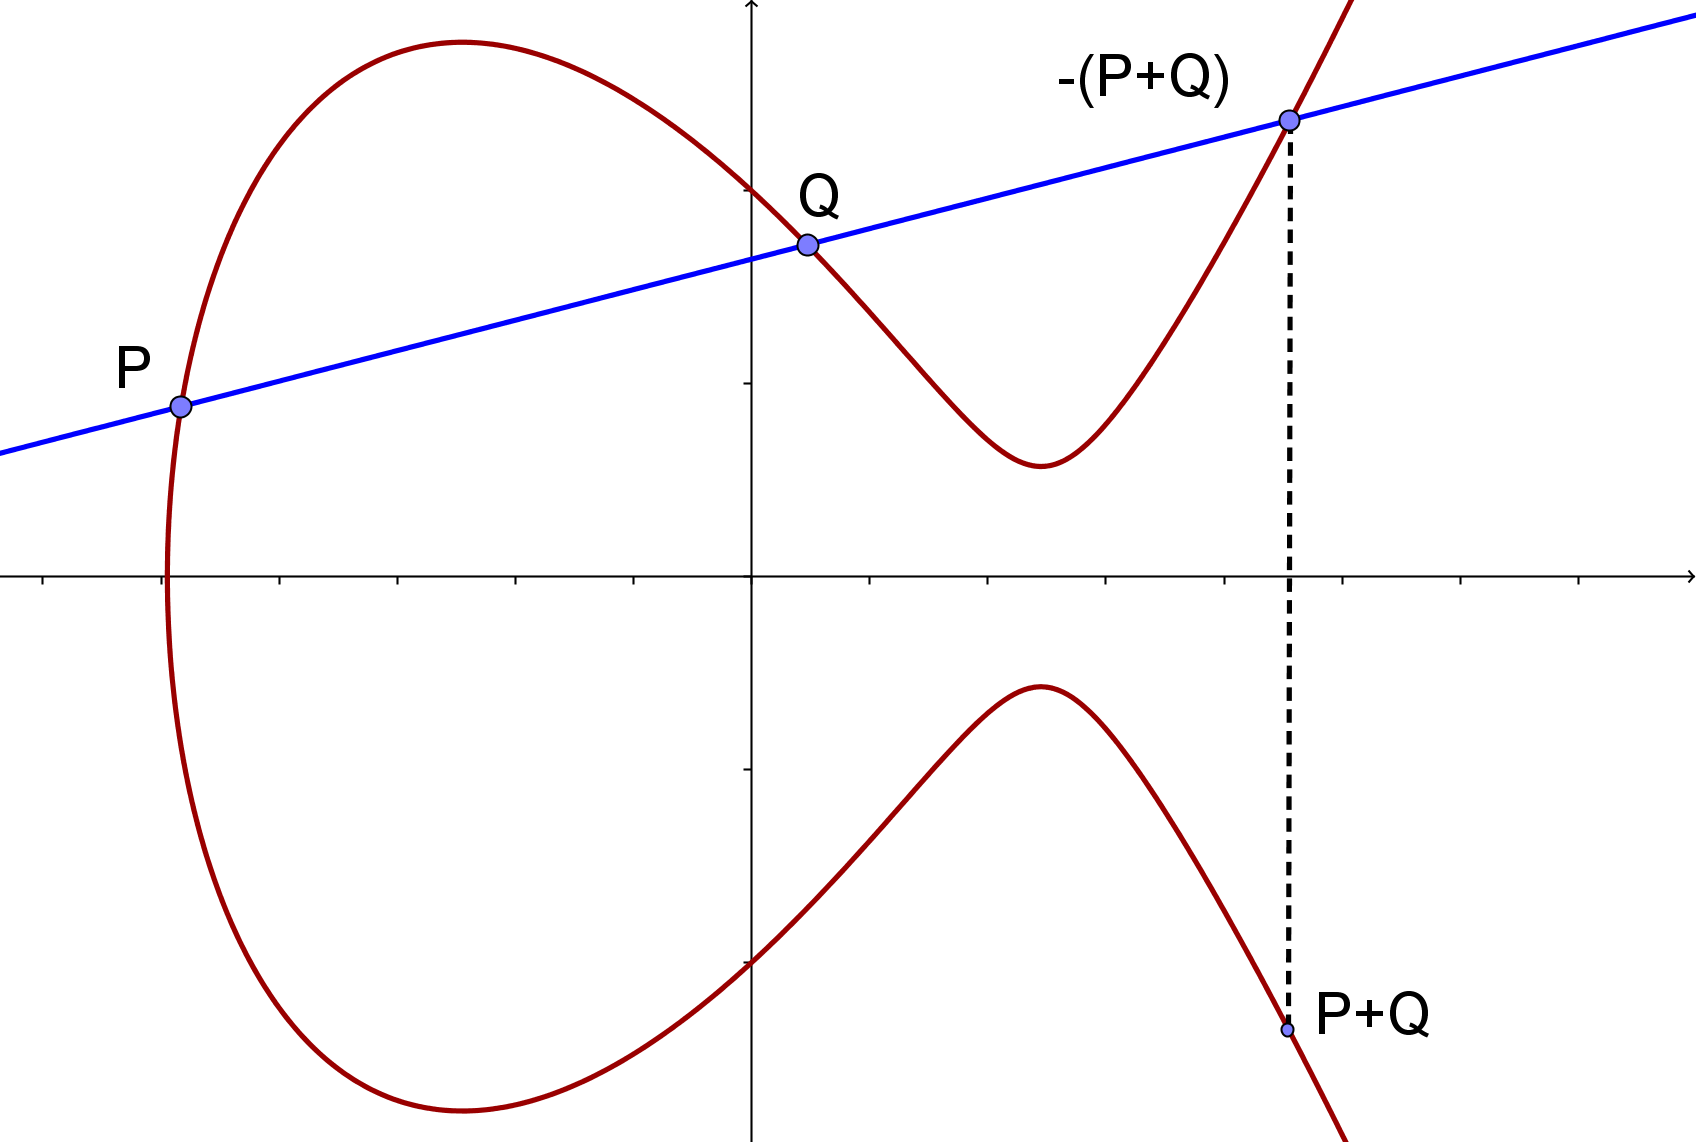
\includegraphics[scale=1]{addition_elliptic_curve.png}
\caption{Dedicated addition on an elliptic curve.}
\label{fig:dedicatedAddition}
\end{minipage}
\hspace{0.5cm}
\begin{minipage}[b]{0.5\linewidth}
\centering
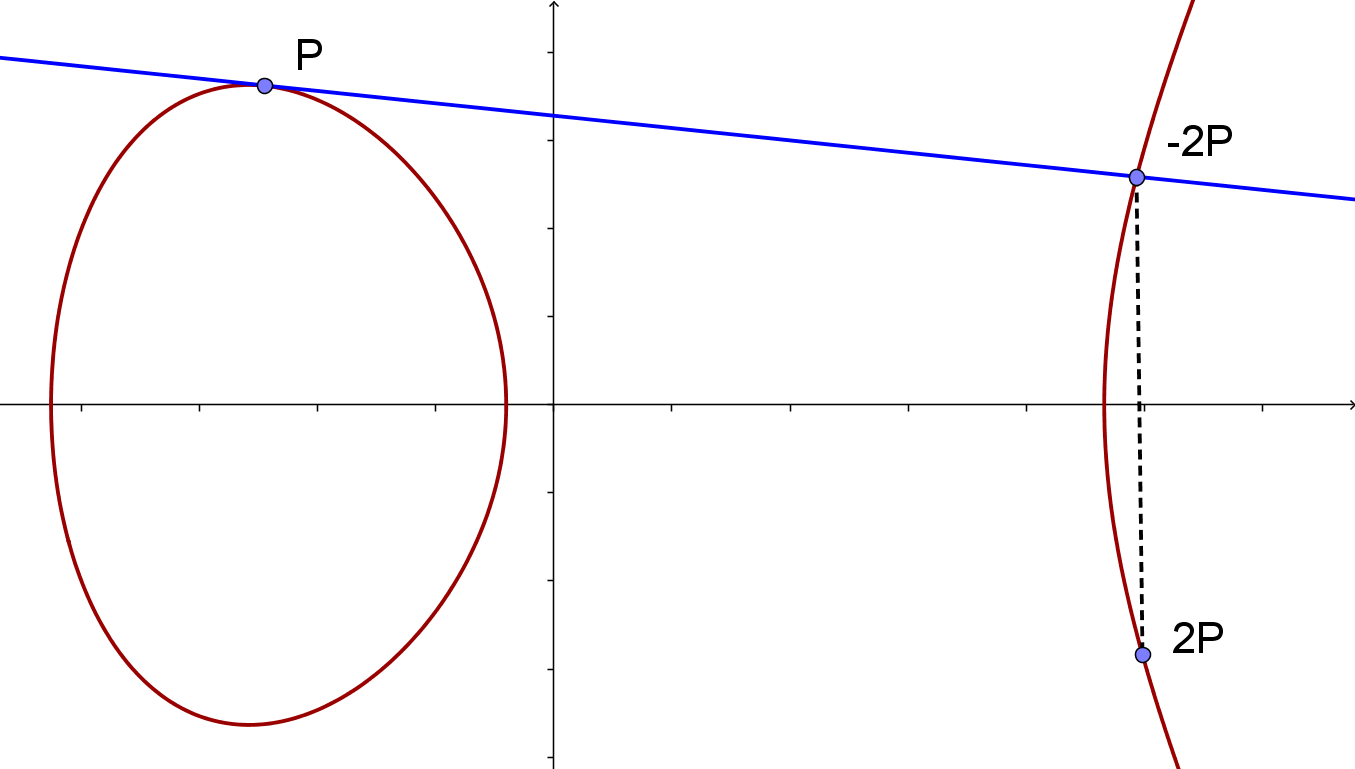
\includegraphics[scale=1.3]{doubling_elliptic_curve.png}
\caption{Doubling on an elliptic curve.\newline}
\label{fig:doubling}
\end{minipage}
\end{figure}
Below is the amazing theorem stating that elliptic curves really are groups; even finitely generated abelian groups. 
\begin{thm}\label{thm:ellipticGroupComposition}
Let $\F$ be a field with $\Char(\F)\neq 3$. Then $(E_{W,a,b,c}(\F),\oplus)$ is a finitely generate abelian group with $\infi$ as neutral element and if $P=(x,y)\in E_{W,a,b,c}(\F)$ the inverse is $-P=(x,-y)$.
\end{thm}
Without confusion we will from now on write $+$ instead of $\oplus$. The hardest thing to prove in the present theorem is the associativity. It can be proven using computer algebra systems such as Maple or if one is masochistic orientated, in hand.  
\begin{rem}\label{rem:groupShortW}
$(E_{W,a,b}(\F),+)$ also satisfy the above theorem with the defined composition. Simply substitute $c=0$ in the formulas. The theorem also apply for general elliptic curves but with a more intricate composition.
\end{rem}
Let $\F_p=\Z/p\Z$. The theorem below is due to Hasse and restrict the curve order of elliptic curves over fields of the form $\F_p$. 
\begin{thm}\label{thm:hasse}
Let $E_{W,a,b}(\F_p)$ be an elliptic curve. Then $\vert E_{W,a,b}(\F_p)\vert \in [p+1-2\sqrt{p},p+1+2\sqrt{2}]$. 
\end{thm}
This theorem is key in the analysis of ECM.
